When using psfrag it is important to use \textbf{latex} and not \textbf{pdflatex} for rendering.

\begin{figure}[htb]
	\centering
	\subfloat{
		\psfrag{a}[c][c]{$\theta$}
		\psfrag{b}[c][c]{$\Sigma$}
		\psfrag{c}[c][c]{Incidence angle}
		\centering
			
\includegraphics[width=70mm]{images/collector_theta-01.eps}
	}\hspace{1cm}
	\subfloat{
		\psfrag{S}[c][c]{S}
		\psfrag{N}[c][c]{N}
		\psfrag{a}[c][c]{$\Sigma$}
		\psfrag{b}[c][c]{$\beta$}
		\psfrag{c}[c][c]{$\phi_\textnormal{S}$}
		\psfrag{d}[c][c]{$\phi_\textnormal{C}$}
		\centering
			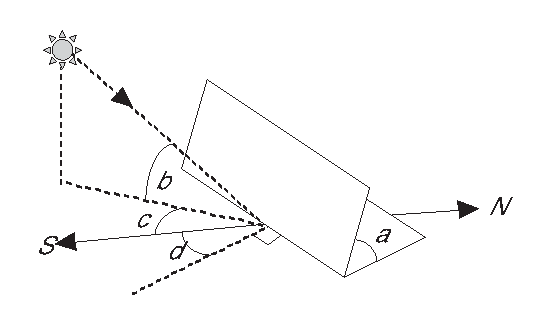
\includegraphics[width=90mm]{images/collector_geometry-01.eps}
	}
	\caption[Geometric conditions between solar irradiation and alignment of the photovoltaic panel]{Geometric conditions between solar irradiation and alignment of the photovoltaic panel \cite{masters04}}
	\label{fig:collector}
\end{figure}